\documentclass[conference]{IEEEtran}
\usepackage[utf8]{inputenc}
\usepackage{amsmath}
\usepackage{amsfonts}
\usepackage{amssymb}
\usepackage{graphicx}
\usepackage{cite}
\usepackage{url}
\usepackage{hyperref}
\usepackage{tikz}
\usetikzlibrary{shapes.multipart, arrows.meta, positioning}


\title{WORKING DRAFT: Multi-Objective Optimization for Automated Guitar Tablature: The gtrsnipe Fretboard Mapper}

\author{
\IEEEauthorblockN{Scott VanRavenswaay}
\IEEEauthorblockA{Email: scottvr@gmail.com}
}

\begin{document}

\maketitle

\begin{abstract}
The task of transcribing music for fretted string instruments like the guitar presents a significant computational challenge known as the ``fretboard mapping problem.'' For any given musical pitch, multiple string and fret combinations may exist, leading to a combinatorial explosion of possible fingerings for a sequence of notes. This paper introduces the gtrsnipe Fretboard Mapper, a novel system designed to solve this problem by framing it as a multi-objective optimization task. The system employs a configurable, weighted scoring function that evaluates potential fingerings based on a combination of physical playability, ergonomic efficiency, and musical context. Key components of our scoring model include penalties for wide fret-stretches, excessive hand movement, and string switching, alongside bonuses for utilizing instrument-specific affordances like open strings, barre chords, and allowing notes to ring out. Furthermore, the mapper incorporates a context-aware algorithm that considers previous fingerings to ensure smooth transitions and a rule-based system for inferring common performance techniques like hammer-ons, pull-offs, and taps. We argue that this multi-constraint approach produces tablature that is not only playable but also stylistically and ergonomically logical, representing a significant improvement over naive or static-rule-based systems in terms of ergonomic and musical coherence.
\end{abstract}

\begin{IEEEkeywords}
Music Information Retrieval, Guitar Tablature, Multi-Objective Optimization, Fretboard Mapping, Automated Transcription
\end{IEEEkeywords}

\section{Introduction}

Music Information Retrieval (MIR) has made significant strides in automated music transcription, particularly in converting audio signals to a symbolic representation like MIDI (Musical Instrument Digital Interface). However, for multi-timbral instruments like the guitar, a MIDI representation is only an intermediate step. The core challenge lies in mapping the abstract pitches of a MIDI event sequence onto the physical constraints of the guitar's fretboard. This is a non-trivial problem due to the instrument's inherent ambiguity.

Unlike a piano, where each pitch corresponds to a single key, a standard-tuned 6-string guitar can produce the same pitch in up to six different locations. For example, the note E4 can be played as the open 1st string, the 5th fret of the 2nd string, the 9th of the 3rd, the 14th of the 4th, and so on. A three-note chord can therefore have dozens of potential fingerings, or voicings. The task of an automated tablature system is to select the single ``best'' fingering for each moment in the music from this vast search space.

This paper details the gtrsnipe Fretboard Mapper, an algorithmic solution to this problem. The system moves beyond naive, greedy approaches by implementing a sophisticated, context-aware scoring function that models the decision-making process of a human guitarist. It balances multiple, often competing, objectives to generate tablature that is both technically feasible and musically coherent.

\begin{figure}[htbp]
\centering
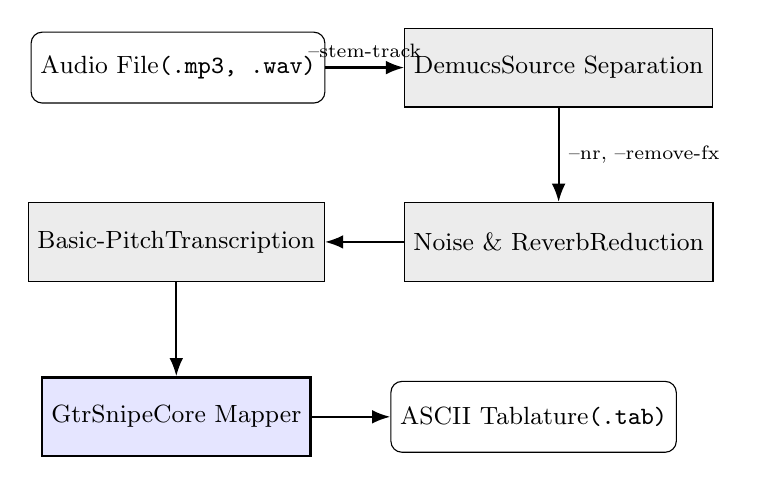
\begin{tikzpicture}[
  node distance=1.2cm and 1.0cm,
  every node/.style={font=\small},
  file/.style={rectangle, draw, rounded corners, minimum width=2.8cm, minimum height=0.9cm, fill=white},
  thirdparty/.style={rectangle, draw, fill=gray!15, minimum width=2.8cm, minimum height=1.0cm},
  gtrsnipe/.style={rectangle, draw, fill=blue!10, thick, minimum width=2.8cm, minimum height=1.0cm},
  output/.style={rectangle, draw, rounded corners, minimum width=2.8cm, minimum height=0.9cm, fill=white},
  arrow/.style={-{Latex}, thick}
]

% First row
\node[file] (audio) {Audio File\\\texttt{(.mp3, .wav)}};
\node[thirdparty, right=of audio] (demucs) {Demucs\\Source Separation};

% Second row (below demucs)
\node[thirdparty, below=of demucs] (nr) {Noise \& Reverb\\Reduction};

% Third row (to left of nr)
\node[thirdparty, left=of nr] (pitch) {Basic-Pitch\\Transcription};

% Fourth row (below pitch)
\node[gtrsnipe, below=of pitch] (mapper) {GtrSnipe\\Core Mapper};

% Final output (to right of mapper)
\node[output, right=of mapper] (tab) {ASCII Tablature\\\texttt{(.tab)}};

% Arrows
\draw[arrow] (audio) -- node[above, font=\scriptsize]{--stem-track} (demucs);
\draw[arrow] (demucs) -- node[right, font=\scriptsize]{--nr, --remove-fx} (nr);
\draw[arrow] (nr) -- (pitch);
\draw[arrow] (pitch) -- (mapper);
\draw[arrow] (mapper) -- (tab);

\end{tikzpicture}
\caption[ ]{End-to-end pipeline of the \texttt{gtrsnipe} system. Third-party tools perform preprocessing; the Core Mapper outputs guitar tablature.}
\label{fig:gtrsnipe_pipeline}
\end{figure}


\section{The Fretboard Mapping Problem: Formulation}

We formally define the Fretboard Mapping Problem as follows:

Given a time-ordered sequence of musical events, $E = \{e_1, e_2, \ldots, e_n\}$, where each event $e_i$ is a tuple of $(time, pitch)$, the goal is to produce a sequence of tablature events $T = \{t_1, t_2, \ldots, t_n\}$, where each $t_i$ is a tuple of $(time, pitch, string, fret)$.

The core of the problem is to assign the optimal string and fret values for each event. This is challenging because:

\textbf{Ambiguity:} Each pitch $p$ maps to a set of fret positions $FP_p = \{(s_1, f_1), (s_2, f_2), \ldots\}$.

\textbf{Combinatorial Complexity:} A chord with pitches $\{p_1, \ldots, p_k\}$ yields candidate fingerings in $FP_{p_1} \times \cdots \times FP_{p_k}$, filtered to disallow duplicate strings.

\textbf{Context Dependency:} The optimal fingering for a chord at time $t$ is dependent on the fingering of the chord at time $t-1$ and, for complex passages, even $t-2$.

The gtrsnipe mapper addresses this by converting the problem into a search for the highest-scoring path through a sequence of possible fingerings.

\section{Methodology: A Multi-Constraint Optimization Approach}

The architecture of the gtrsnipe mapper is built around the \texttt{GuitarMapper} class, which operates on a \texttt{MapperConfig} data structure. This configuration holds the weights and thresholds for every parameter in the scoring algorithm, allowing for fine-grained control over the final output. The process is divided into three main stages: Search Space Generation, Scoring, and Technique Inference.

\subsection{Search Space Generation}

The first step, handled by the \texttt{\_build\_pitch\_maps} method, is to generate a lookup table (\texttt{pitch\_to\_positions}) that maps every playable MIDI pitch to a set of all possible \texttt{FretPosition} objects. This process is initialized based on the instrument's tuning, number of frets, and any specified capo position, making the system adaptable to a wide variety of instruments and playing styles (e.g., standard 6-string, 7-string, bass, baritone).

\subsection{The Multi-Objective Scoring Function}

The core of our methodology is the \texttt{\_score\_fingering} function. For any given fingering (a collection of \texttt{FretPosition} objects), this function calculates a score based on several weighted criteria. A higher score indicates a more desirable fingering. The final score $S_{total}$ is a summation of several component scores:

\begin{equation}
S_{total} = S_{shape} + S_{position} + S_{transition} + S_{musical}
\end{equation}

\subsubsection{Internal Shape Score ($S_{shape}$)}
This score evaluates the ergonomic feasibility of a single chord shape in isolation.

\textbf{Fret Span Penalty:} It penalizes fingerings that require an uncomfortable or impossible stretch. The penalty is proportional to the distance between the highest and lowest frets used in the chord.

\begin{equation}
S_{span} = -w_{fret\_span} \times (\max(F) - \min(F))
\end{equation}

where $F$ is the set of frets in the fingering and $w_{fret\_span}$ is a configurable penalty weight. A hard cutoff (\texttt{unplayable\_fret\_span}) immediately disqualifies fingerings that exceed a defined span.

\textbf{Barre Bonus/Penalty:} It adjusts the score based on the use of a ``barre'' (using one finger to press multiple strings at the same fret). This can be a bonus for economy of motion or a penalty if barre chords are to be avoided.

\subsubsection{Positional Score ($S_{position}$)}
This score evaluates where the fingering is located on the fretboard.

\textbf{Sweet Spot Bonus:} Rewards fingerings that fall within a defined ``sweet spot'' on the neck (e.g., frets 0-12), which is often more comfortable for open chords and melodic playing.

\textbf{High Fret Penalty:} Applies a penalty for playing high on the neck, which can be further multiplied if occurring on the lower-pitched strings, a common heuristic for avoiding ``muddy'' sounding voicings.

\subsubsection{Transition Score ($S_{transition}$)}
This crucial component makes the algorithm context-aware by evaluating the cost of moving from the previous fingering (\texttt{prev\_fingering}) to the current one.

\textbf{Movement Penalty:} Penalizes large horizontal shifts of hand position up or down the neck.

\textbf{String Switch Penalty:} Penalizes fingerings that involve changing sets of strings, encouraging more fluid, contiguous playing.

\textbf{Diagonal Span Constraint:} A key innovation (\texttt{count\_fret\_span\_across\_neighbors}) that penalizes fingerings where the stretch between a note in the current fingering and a note in the previous fingering is unplayable. This prevents awkward jumps that are not captured by analyzing chords in isolation.

\subsubsection{Musical and Stylistic Score ($S_{musical}$)}
This component rewards choices that align with common musical practices.

\textbf{Let-Ring Bonus:} Awards a bonus to fingerings that leave strings used by the previous fingering open, allowing those notes to sustain naturally. This is critical for emulating styles like classical and folk guitar.

\textbf{Open String Preference:} Penalizes using a fretted note when the same pitch could be played as an open string, controlled by the \texttt{prefer\_open} flag and \texttt{fretted\_open\_penalty}.

\subsection{Technique Inference}

After the optimal fret positions are determined, a final pass (\texttt{\_infer\_techniques\_from\_positions}) analyzes the resulting sequence to infer performance articulations. By examining the time delta, pitch delta, and string continuity between consecutive notes, it applies labels for hammer-ons, pull-offs, and taps, adding a layer of musical expressiveness to the final tablature. This is achieved through a set of heuristics, such as identifying a fast-ascending pitch sequence on a single string as a hammer-on.

\section{Proposed Evaluation Framework: An Ablation Study}

We define an ablation study to validate our model and understand the contribution of each parameter. An ablation study involves removing or altering individual components of the system to observe the impact on the output quality.

As noted in preliminary analysis: ``Your documentation captures exactly the kind of systematic parameter exploration that academic research needs... The narrative of `systematic improvement through parameter adjustment' is exactly what ablation studies should demonstrate.''

Our proposed study would consist of:

\textbf{Baseline Establishment:} Generate tablature for a corpus of test pieces using default \texttt{MapperConfig} parameters. This serves as the control group.

\textbf{Single-Parameter Sensitivity Analysis:} For each key parameter (e.g., \texttt{let\_ring\_bonus}, \texttt{movement\_penalty}, \texttt{fret\_span\_penalty}), generate new tablatures while varying only that parameter across a predefined range.

\textbf{Evaluation Metrics:}

\textit{Quantitative Metrics:} We will measure computational metrics like Average Fret Span, Hand Position Changes per Measure, and String Switch Frequency.

\textit{Qualitative Metrics:} The generated tablatures will be presented to a panel of experienced guitarists who will rate them on a 1-10 Likert scale for Playability and Musical Authenticity.

\textbf{Comparative Analysis:} The results will be compared against both the baseline and professionally published, human-generated tablatures of the same pieces.

This study will allow us to quantify the impact of each heuristic and develop optimized \texttt{MapperConfig} profiles for different musical genres (e.g., a ``Classical'' profile with a high \texttt{let\_ring\_bonus} vs. a ``Metal'' profile with a high \texttt{string\_switch\_penalty}).

\section{Conclusion and Future Work}

The gtrsnipe Fretboard Mapper provides a robust and highly configurable framework for solving the complex problem of automated guitar tablature generation. By treating the task as a multi-objective, context-aware optimization problem, it produces fingerings that are ergonomically and musically superior to those from simpler systems.

Future work will focus on two primary areas. First, we plan to implement the proposed ablation study to empirically validate the model and its parameters. Second, we will explore replacing the manually-weighted scoring function with a machine learning model. By training a model on a large corpus of high-quality, human-created tablatures, we could learn the optimal parameter weights automatically, potentially uncovering more subtle and complex relationships that define a ``good'' fingering.

\section*{Acknowledgments}
The author would like to thank Claude.ai for valuable feedback on the experimental design and academic framing of this work, and Gemini 2.5 Pro for the help formalizing and formatting the mathematical representation of how gtrsnipe works, as well as ChatGPT 4o for providing feedback on drafts along the way.

\begin{thebibliography}{1}

\bibitem{ref1}
[Future references to related work in MIR, guitar tablature generation, and multi-objective optimization would go here]

\end{thebibliography}

\end{document}